\documentclass[xcolor=dvipsnames,compress]{beamer}
% \documentclass[xcolor=dvipsnames,compress,handout]{beamer}
% \documentclass[xcolor=dvipsnames,compress,trans]{beamer}
\usepackage[utf8]{inputenc}
\usepackage{default}
\usepackage[T1]{fontenc}
\usepackage{ngerman}
\usepackage{amssymb, amsmath}
\usepackage{xfrac}
\usepackage{hyperref}
\usepackage{eurosym}
\usepackage{siunitx}
\sisetup{
  separate-uncertainty = true,
  multi-part-units = brackets,
  open-bracket = (,
  close-bracket = ),
  exponent-product = \cdot,
  add-decimal-zero = true,
  add-integer-zero = true,
  per-mode         =   reciprocal,
%   prefixes-as-symbols = true,
%   output-decimal-marker = {,},
  table-figures-uncertainty = 1,
  load-configurations = binary,
  load-configurations = abbreviations,
  sticky-per
}

% \setbeamercovered{transparent}

% Design, Colors
\usecolortheme[named=NavyBlue]{structure}
\setbeamercolor{palette secondary}{bg=Blue,fg=white} % unten, subsection bar
\setbeamercolor{palette tertiary}{bg=black,fg=white} % bar oben, title bar
\setbeamercolor{titlelike}{bg=NavyBlue,fg=white}
\setbeamercolor{block title}{bg=NavyBlue,fg=white}
\setbeamercolor{block body}{bg=NavyBlue!10}
\setbeamercolor{block title example}{bg=OliveGreen,fg=white}
\setbeamercolor{block body example}{bg=OliveGreen!10}
% Design

\useinnertheme{rectangles}
\useoutertheme[subsection=true]{miniframes}
\setbeamertemplate{navigation symbols}{}
\setbeamertemplate{footline}
% \setbeamercolor{alerted text}{fg=red}
% \setbeamercolor{block title defintion}{bg=black,fg=white}
{%
  \begin{beamercolorbox}[colsep=1.5pt]{upper separation line foot}
  \end{beamercolorbox}
  \begin{beamercolorbox}[ht=2.5ex,dp=1.125ex,%
    leftskip=.3cm,rightskip=.3cm plus1fil]{title in head/foot}%
    {\usebeamerfont{title in head/foot}\insertshorttitle}%
    \,
    {\usebeamerfont{author in head/foot}(\insertshortauthor)}%
    \hfill
    {\usebeamerfont{framenumber in head/foot}\textbf{\insertframenumber}}%
  \end{beamercolorbox}%
  \begin{beamercolorbox}[colsep=1.5pt]{lower separation line foot}
  \end{beamercolorbox}
}
% \beamertemplatetransparentcoveredhigh
% \beamertemplatetransparentcovereddynamicmedium 

\title[KDE on Linux]{How to work with Linux and KDE as a scientist}
\author{Thomas Murach \and Robert Riemann}
\institute[HU Berlin]{Humboldt-Universität zu Berlin}
\date{21. März 2012}
\titlegraphic{
\includegraphics[width=0.25\linewidth]{siegel}}

\hypersetup
{
	pdfauthor	=	{Thomas Murach, Robert Riemann},
	pdftitle	=	{How to work with Linux and KDE as a scientist}
}


\begin{document}

% \renewcommand{\inserttotalframenumber}{17}

\logo{
\includegraphics[height=1cm]{siegel.pdf}}
% \frame{
% \titlepage
% }

\begin{frame}[plain]
\titlepage
\end{frame}
% 
% \frame{
% \frametitle{Gliederung}
% \tableofcontents
% }
% \section{Progress}

\section{Best Practice}

\frame{
\frametitle{Plan und Todo}
TODO:
\begin{itemize}
  \item Linux ist quasi virenfrei :)
  \item Installation (nach kurzer Einleitung, erwähnen: versch. Distros existieren etc.) durchführen
  \item einleitende Worte zu KDE
  \item Softwarestruktur in Linux + Paketmanager, zu Yast hinführen (-> exemplarisch Roberts Repo hinzufügen)
  \item generell: coole Programme vorstellen (kurz jeweils) (Bsp.: ssh (+scp,sshfs,...); kile(?); kdevelop; mathe-programme; bash(?); git; yakuake; convert
\end{itemize}
}

\subsection{SSH}
\frame{
\frametitle{Entferntes Arbeiten: ssh}
\begin{itemize}
  \item man kann bspw. Programme auf den Uni-Rechnern laufen lassen, die man selbst nicht installiert hat (z.B. Maple o.ä.)
  \item oder: Dateien einfach von Pool-Rechnern auf seinen PC kopieren, wenn man zu Hause weiter arbeiten will
\end{itemize}
}

\frame{
\frametitle{Wie geht das?}
Anmelden in Konsole:\\
\begin{center}
  \texttt{ssh user@pool1.physik.hu-berlin.de}
\end{center}
Dateien kopieren:\\
% \begin{center}
  \texttt{scp foo.bar user@pool1.physik.hu-berlin.de:path}\\
  \texttt{scp user@pool1.physik.hu-berlin.de:path/file.txt .}
% \end{center}
}

\frame{
\frametitle{Sicherheitsaspekte}
\begin{itemize}
  \item gut: Authentifizierung mit verschlüsseltem Key
  \item Key erzeugen:\\
        \begin{center}
          \texttt{ssh-keygen -b 1024 -t dsa}		% besser rsa?
        \end{center}
  \item Public Key nach $\sim$/.ssh kopieren und an Datei $\sim$/.ssh/authorized\_keys anhängen:\\
        \begin{center}
          \texttt{ssh-copy-id user@pool1. ...}
        \end{center}
  \item Rechte anpassen:\\
        \begin{center}
          \texttt{chmod 600 $\sim$/.ssh/authorized\_keys}
        \end{center}
  \item schließlich: ssh-agent verwenden, um Passwort nur einmal eingeben zu müssen (pro Sitzung):
        \begin{center}
          \texttt{ssh-add}
        \end{center}
\end{itemize}
}

\subsection{kleine Helfer}

\frame{
\frametitle{Bildkonvertierung mit \texttt{convert}}
um Bilder zu konvertieren (z.B. jpg $\rightarrow$ png):
\begin{center}
  \texttt{convert a.jpg b.png}
\end{center}
(benötigt das Paket „ImageMagick“)
}

\frame{
\frametitle{Vektorgraphiken konvertieren}
Um Vektorgraphiken zu konvertieren, gibt es viele kleine, spezielle Programme:
\texttt{ps2pdf} bzw. \texttt{pstopdf}, \texttt{epstopdf}, etc.
}

\begin{frame}{Zwischenablage unter Linux}
  \begin{itemize}
    \item Wie Windows: \texttt{<Strg+C>} und \texttt{<Strg+V>}
    \item In der Konsole und fast allen Linux-Programmen zusätzlich: \\
          Markieren (Kopieren) und Mittle Maustaste (Einfügen)
    \item Verwaltung der History der letzten Einträge in der Zwischenablage
          durch \textit{Klipper} (Schere im System-Abschnitt)
  \end{itemize}
\end{frame}

\begin{frame}{Programme Abschießen}
  Für den unwahrscheinlichen Fall, dass etwas nicht geht:
  \begin{itemize}
    \item In der Konsole: \\ \texttt{killall -9 app-name} \\ \textit{oder} \\
    \texttt{<Strg>+<C>}
    \item Graphisch: \\ \texttt{<Strg> + <Alt> + <Esc> +} Linksklick \\
          \textit{oder} \\
          mit dem Linux-Taskmanager Systemmonitor \texttt{ksysguard}
    \item Den Benutzer ohne weitere Rückfragen ausloggen: \\
          $2 \times$\texttt{<Strg>+<Alt>+<Backspace>}
  \end{itemize}
\end{frame}

\section{Programme}

\begin{frame}{All-In-One Messenger Kopete}
  \begin{columns}
    \begin{column}{0.45\textwidth}
      \begin{itemize}
        \item Ende-zu-Ende Verschlüsselung (OTR)
        \item ICQ, MSN, Jabber, Facebook, StudiVZ, Google, AIM
        \item \LaTeX-Support
        \item Bilder-Vorschau
      \end{itemize}      
    \end{column}
    \begin{column}{0.55\textwidth}
      \begin{figure}
        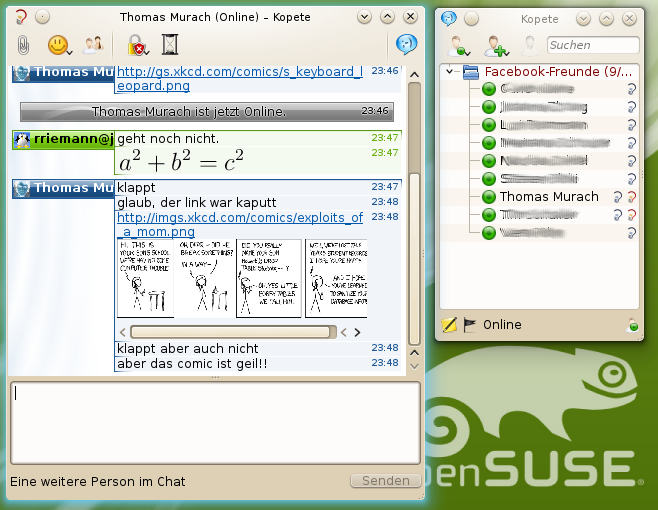
\includegraphics[bb=0 0 493 382,keepaspectratio=true,width=\textwidth]{kopete}
        % kopete.png: 658x510 pixel, 96dpi, 17.41x13.49 cm, bb=0 0 493 382
        \caption{Kopete}
      \end{figure}
    \end{column}
  \end{columns}
\end{frame}

\begin{frame}{Everywhere-Dateimanager Dolphin}
  \begin{columns}
    \begin{column}{0.45\textwidth}
      \begin{itemize}
        \item Tabs, 2-Spalten, Dateibaum, Vorschau, etc.
        \item KIO: ftp, sftp, NFS, webdav und Windows-Shares (Samba)
        \item Datein filtern, Volltextsuche mit Cache
        \item Konsole-Integration
      \end{itemize}      
    \end{column}
    \begin{column}{0.55\textwidth}
      \begin{figure}
        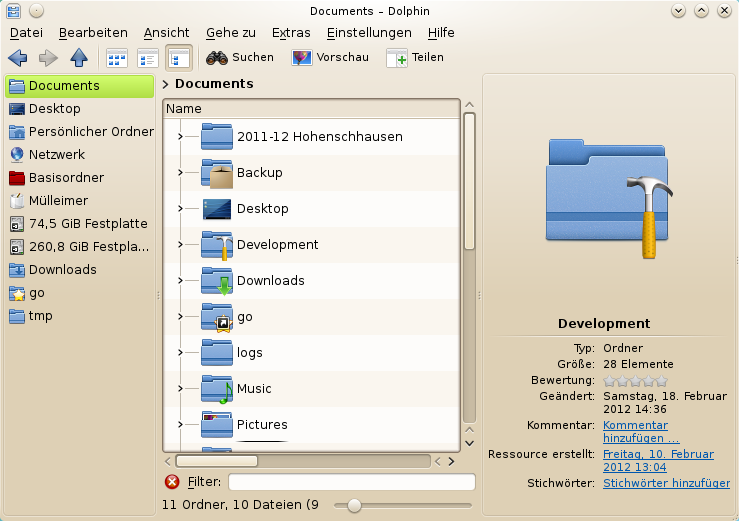
\includegraphics[keepaspectratio=true,width=\textwidth]{dolphin}
        \caption{Dolphin}
      \end{figure}
    \end{column}
  \end{columns}
\end{frame}

\begin{frame}{Mails mit KMail}
  \begin{columns}
    \begin{column}{0.3\textwidth}
      \begin{itemize}
        \item Offline-IMAP
        \item Volltextsuche
        \item Integrierte PGP/SMIME-Verschlüsselung
        \item Anzeige der Mails nach Datum und Betreff
      \end{itemize}      
    \end{column}
    \begin{column}{0.7\textwidth}
      \begin{figure}
        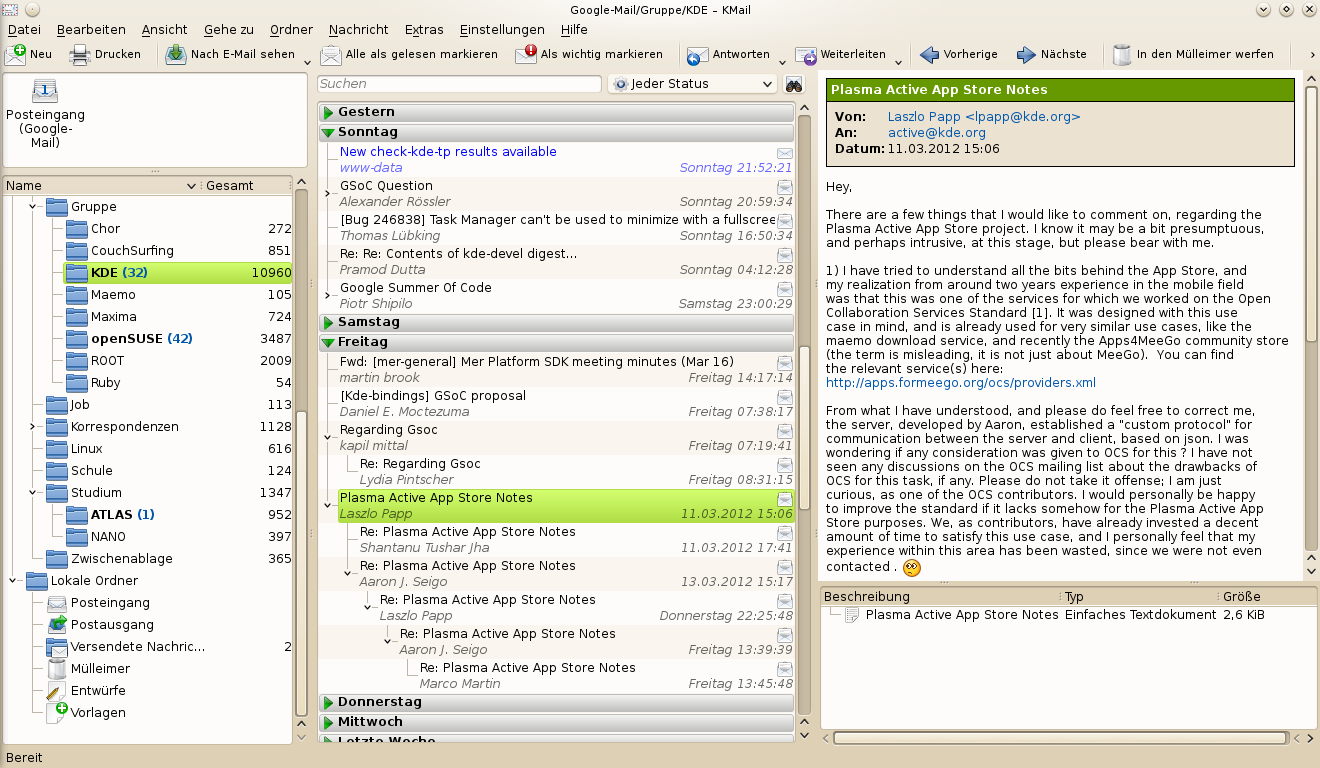
\includegraphics[keepaspectratio=true,width=\textwidth]{kmail}
        \caption{KMail}
      \end{figure}
    \end{column}
  \end{columns}
\end{frame}

\begin{frame}{wxMaxima}
  \begin{figure}
    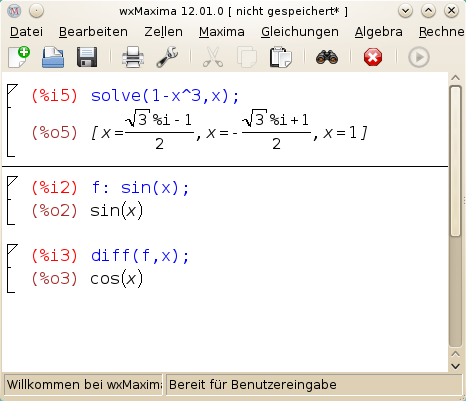
\includegraphics[keepaspectratio=true,width=0.65\textwidth]{wxmaxima}
    \caption{Maple (Mathematica) Klon: wxMaxima}
  \end{figure}
\end{frame}

\begin{frame}{QtOctave}
  \begin{figure}
    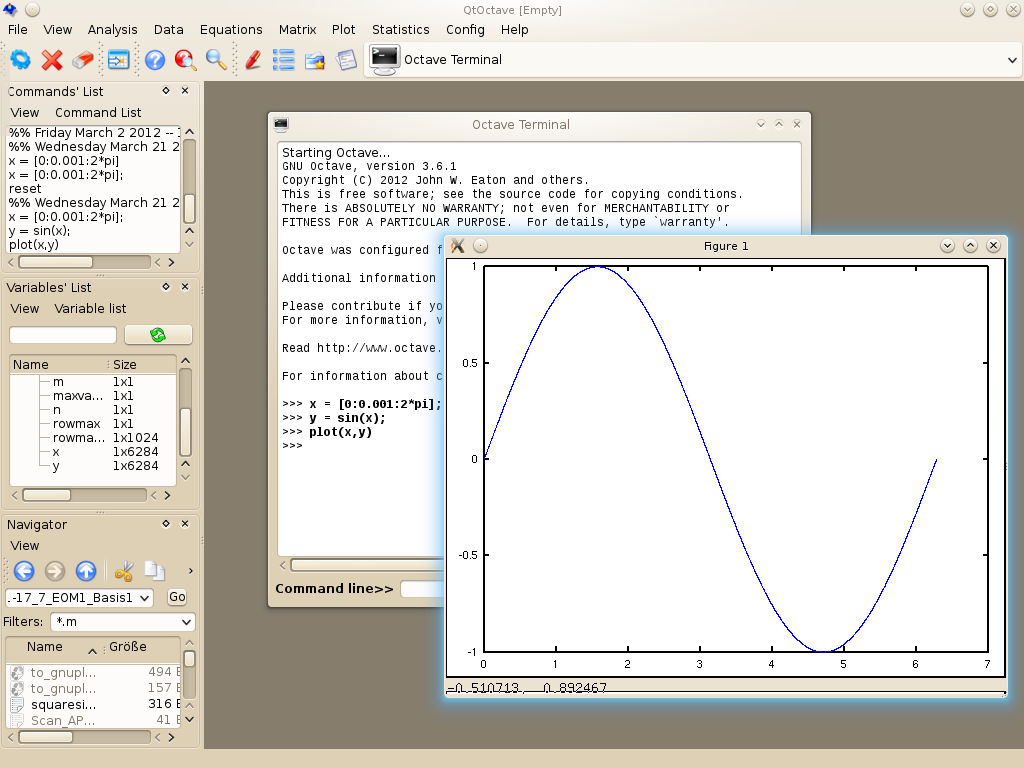
\includegraphics[keepaspectratio=true,width=0.75\textwidth]{qtoctave}
    \caption{Matlab Klon: QtOctave}
  \end{figure}
\end{frame}

\begin{frame}{Kile und Okular}
  \begin{figure}
    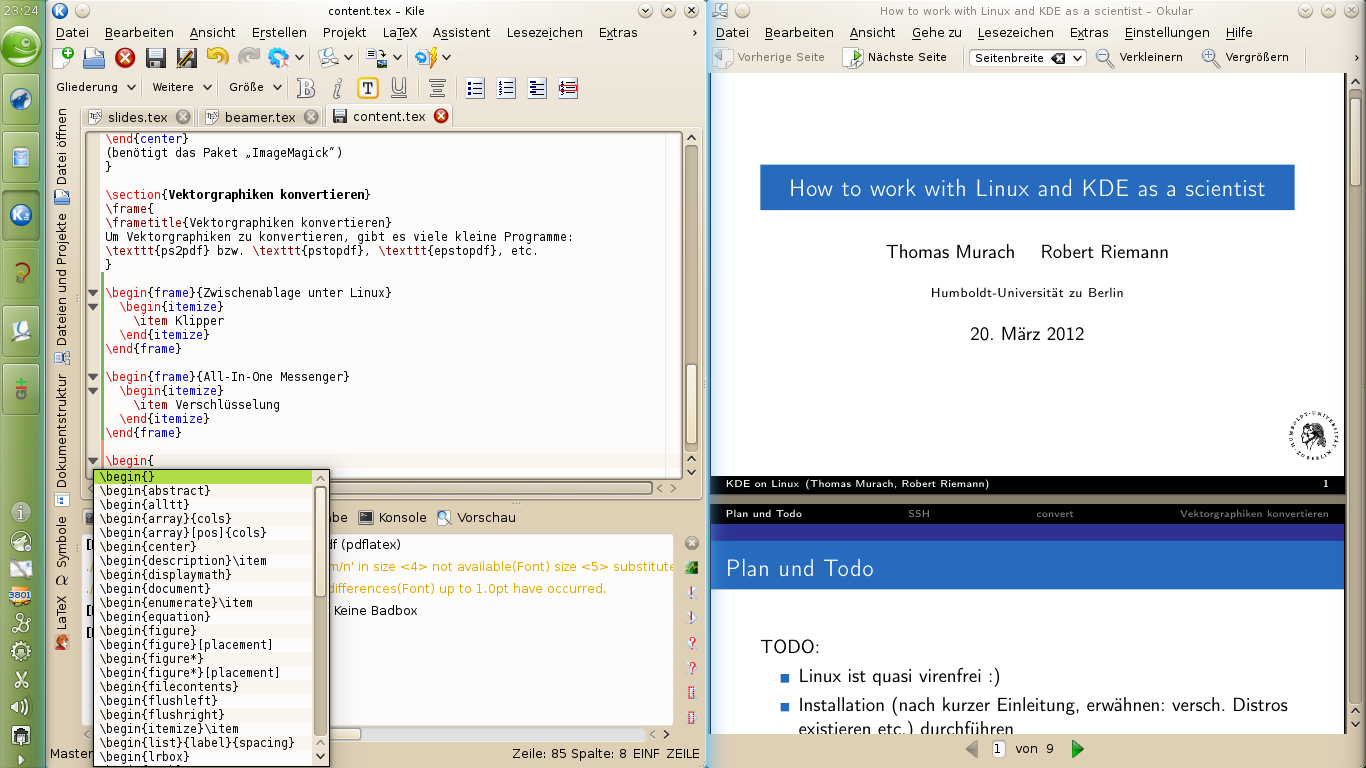
\includegraphics[keepaspectratio=true,width=0.95\textwidth]{kile}
    \caption{\LaTeX-Editor Kile und PDF-Programm Okular}
  \end{figure}
\end{frame}

\begin{frame}{Globale Systemeinstellungen mit YaST2}
  \begin{figure}
    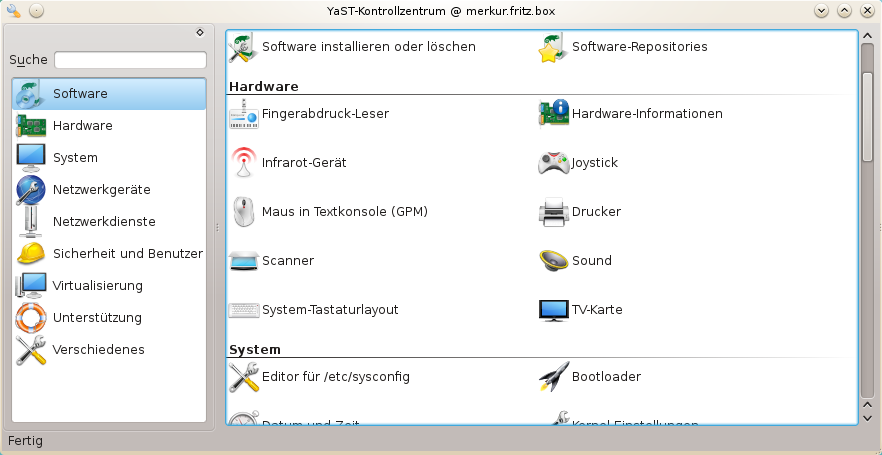
\includegraphics[keepaspectratio=true,width=0.95\textwidth]{yast2}
    \caption{Systemeinstellungen unter Linux: YaST2}
  \end{figure}
\end{frame}

\begin{frame}{Mit Git Arbeiten}
  \begin{figure}
    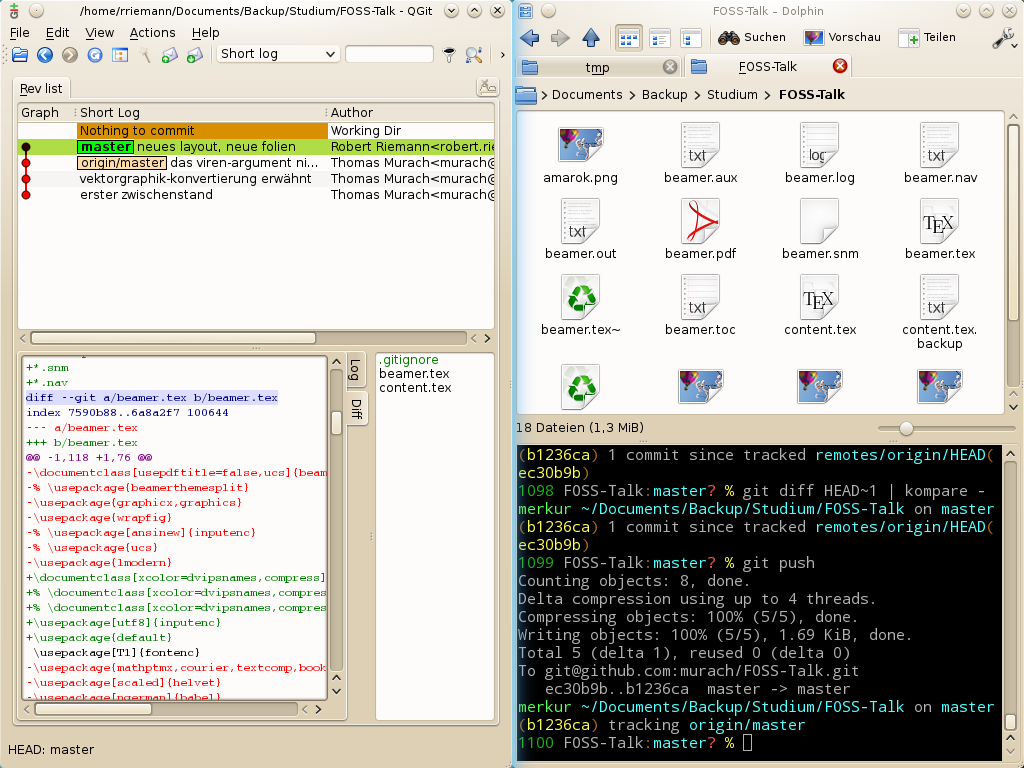
\includegraphics[keepaspectratio=true,width=0.75\textwidth]{qgit_dolphin}
    \caption{QGit und Dolphin mit aktiver Konsolenintegration}
  \end{figure}  
\end{frame}

\begin{frame}{Mit KRunner Arbeiten}
  \begin{columns}
    \begin{column}{0.5\textwidth}
      \begin{itemize}
        \item Aufruf: \texttt{<Alt>+<F2>}
      \end{itemize}
      \begin{figure}
        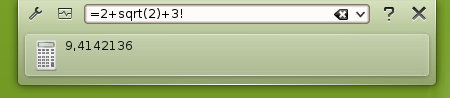
\includegraphics[keepaspectratio=true,width=0.75\textwidth]{krunner}
        \caption{Taschenrechner}
      \end{figure}  
      \begin{figure}
        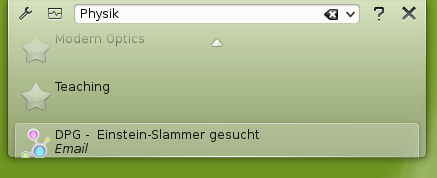
\includegraphics[keepaspectratio=true,width=0.75\textwidth]{krunner2}
        \caption{Volltextsuche}
      \end{figure}
    \end{column}
    \begin{column}{0.5\textwidth}
      \begin{figure}
        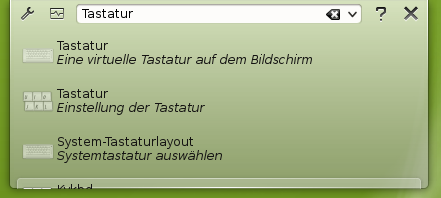
\includegraphics[keepaspectratio=true,width=0.75\textwidth]{krunner3}
        \caption{Einstellungen Finden}
      \end{figure}  
      \begin{figure}
        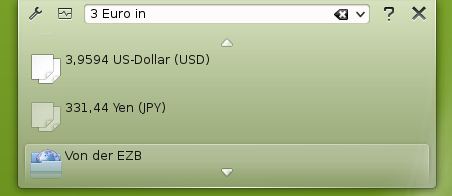
\includegraphics[keepaspectratio=true,width=0.75\textwidth]{krunner4}
        \caption{Einheiten Umrechnen}
      \end{figure}
    \end{column}
  \end{columns}
\end{frame}

\begin{frame}{Editor Kate}
  \begin{columns}
    \begin{column}{0.35\textwidth}
      \begin{itemize}
        \item Hervorhebungen für \textit{alle} Sprachen
        \item Tabs
        \item beliebiges unterteilen der Ansicht
        \item Konsole
        \item Code-Folding
        \item eigene Befehle und Plugins
      \end{itemize}
    \end{column}
    \begin{column}{0.65\textwidth}
      \begin{figure}
        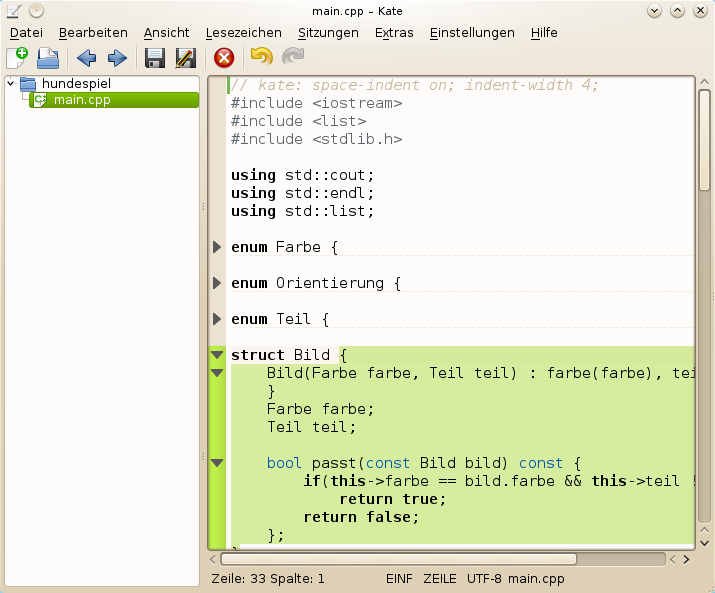
\includegraphics[keepaspectratio=true,width=\textwidth]{kate}
        \caption{Kate}
      \end{figure}      
    \end{column}
  \end{columns}
\end{frame}

\begin{frame}{Uni-WLAN eduroam}
  \begin{columns}
    \begin{column}{0.5\textwidth}
      Einstellungen
      \begin{itemize}
        \item WPA2 Enterprise
        \item TTLS
        \item anonymous@physik.hu-berlin.de
        \item CA-Zertifikat (*.crt) der Telekom
        \item Benutzer: E-Mail-Adresse
        \item Passwort: E-Mail-Passwort
      \end{itemize}
    \end{column}
    \begin{column}{0.5\textwidth}
      \begin{figure}
        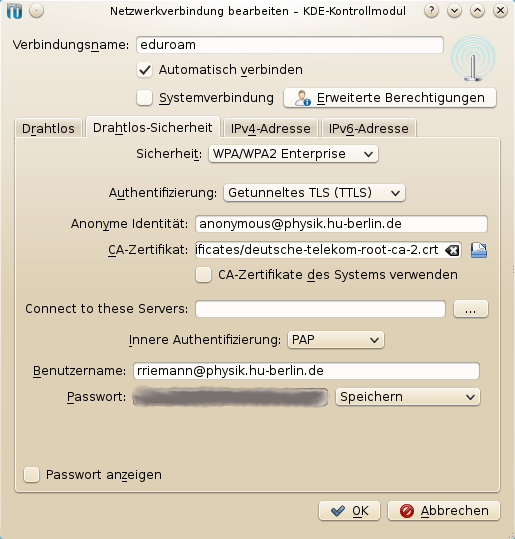
\includegraphics[keepaspectratio=true,width=0.9\textwidth]{eduroam}
        \caption{WLAN eduroam einrichten}
      \end{figure}
    \end{column}
  \end{columns}
\end{frame}

\begin{frame}[fragile]{Shell-Programmierung}
  \lstset{language=bash,
          numbers=left,
          numberstyle=\tiny,
          showstringspaces=false,
          aboveskip=-40pt,
          frame=leftline
  }
  \vspace{2em}
          
  \begin{lstlisting}[caption={Beispiel zur Audio/Video Konvertierung},captionpos=b]
#!/usr/bin/zsh

# source: https://gist.github.com/1385642
#         git://gist.github.com/1385642.git

for file in ./**/*.wma; do
  ffmpeg -i $file -f ogg -acodec libvorbis \
         -ab 128k ${file%.*}.ogg
  mkdir -p ./old_wma/${file%/*}
  mv $file ./old_wma/${file}
done
   \end{lstlisting}
 
\end{frame}


\begin{frame}{All-In-One Messenger}
  \begin{columns}
    \begin{column}{0.5\textwidth}
      
    \end{column}
    \begin{column}{0.5\textwidth}
      
    \end{column}
  \end{columns}
\end{frame}



\end{document}